%\documentclass{article}
%\usepackage{tikz}
%\begin{document}
	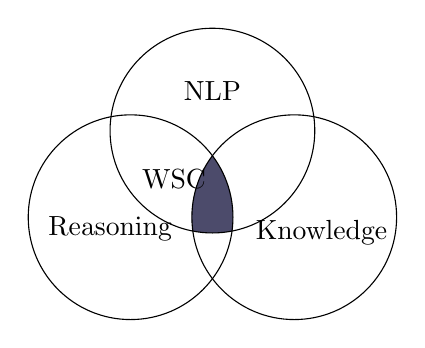
\begin{tikzpicture}
	\definecolor{Psy}{HTML}{4C4B6B}
	 \begin{scope}%[blend group=soft light]
	 
	 \def\firstcircle{( 90:0.5) circle (1.3cm)}
	 \def\secondcircle{(210:1.2) circle (1.3cm)}
	 \def\thirdcircle{(330:1.2) circle (1.3cm)}
	    \fill[white]  \firstcircle;
		 \fill[white] \secondcircle;
		 \fill[white] \thirdcircle;
		 
			 
		  \begin{scope}
		\clip \firstcircle;
		\clip \secondcircle;
		\fill[Psy] \thirdcircle;
		\end{scope}
			 
		 \draw \firstcircle;
		 \draw \secondcircle;
		 \draw \thirdcircle;
		 
		 \node at ( 90:1)    {NLP};
		 \node at (210:1.5)    {Reasoning};
		 \node at (330:1.6)    {Knowledge};
		 \node at (193:0.5) {WSC};
		 
		 
		 
	\end{scope}	 
	\end{tikzpicture}
%\end{document}